% -----------------------------------------------------------------------------
%
% Copyright (c) 2017 Sam Cox, Roberto Sommariva
%
% This file is part of the AtChem2 software package.
%
% This file is covered by the MIT license which can be found in the file
% LICENSE.md at the top level of the AtChem2 distribution.
%
% -----------------------------------------------------------------------------

\chapter{Model Setup} \label{ch:setup}

% -------------------------------------------------------------------- %
\section{Chemical Mechanism} \label{sec:chemical-mechanism}

The chemical mechanism is the core of an atmospheric chemistry
model. In AtChem2, the chemical mechanism file is written in FACSIMILE
format and has the extension \texttt{.fac}. The format is used to
describe chemical reactions in the commercial FACSIMILE Kinetic
Modelling Software; for historical reasons, the software and the
format have often been used in conjunction with the MCM. The
\href{http://mcm.york.ac.uk/extract.htt}{extraction tool} on the
MCM website can generate \texttt{.fac} files in FACSIMILE format that
can be directly used in AtChem2 (Sect.~\ref{subsec:mcm-extraction}).

\subsection{FACSIMILE format} \label{subsec:facsimile-format}

Chemical reactions are described in FACSIMILE format using the
following notation:

\begin{verbatim}
% k : A + B = C + D ;
\end{verbatim}

where \texttt{k} is the rate coefficient, \texttt{A} and \texttt{B}
are the reactants, \texttt{C} and \texttt{D} are the products. A
reaction starts with the \texttt{\%} character and ends with the
\texttt{;} character. The \texttt{:} character separates the rate
coefficient from the reactants and products of the chemical
reaction. The rate coefficient (\texttt{k}) is a constant number or, more
commonly, is calculated as a function of other variables, such as
temperature (\texttt{TEMP}), air density (\texttt{M}), water vapour
(\texttt{H2O}) and other environment variables
(Sect.~\ref{sec:environment-variables}).

Comments can be inserted in the \texttt{.fac} file to document and
annotate the chemical mechanism: in FACSIMILE format, comments are
enclosed between the \texttt{*} and \texttt{;} characters and are
ignored by the compilation scripts. A basic chemical mechanism, with
comments and calculated rate coefficients, has the following format:

\begin{verbatim}
* Tropospheric O3-NOx cycle ;
* Kinetic data from Atkinson et al., ACP, 2004 ;
*;
% J_NO2                      : NO2 = NO + O ;
% 5.6D-34*M*(TEMP/300)@-2.6  : O + O2 = O3 ;
% 1.4D-12*EXP(-1310/TEMP)    : NO + O3 = NO2 + O2 ;
\end{verbatim}

The photolysis rate of \cf{NO2} (\texttt{J\_NO2}) in the example above
is calculated by AtChem2 as function of latitude, longitude and solar
zenith angle (Sect.~\ref{subsec:calculated-photolysis-rates}).
Complex mathematical expressions can be used to calculate the rate
coefficients, in which case they have to be defined before the
chemical reactions that use them (typically, these are combination and
dissociation reactions). For example:

\begin{verbatim}
* Formation of nitric acid (HNO3) in the gas-phase ;
*;
* Rate coefficient (Atkinson et al., ACP, 2004) ;
K80 = 3.3D-30*M*(TEMP/300)@-3.0 ;
K8I = 4.1D-11 ;
KR8 = K80/K8I ;
FC8 = 0.4 ;
NC8 = 0.75-1.27*(LOG10(FC8)) ;
F8 = 10@(LOG10(FC8)/(1+(LOG10(KR8)/NC8)**2)) ;
KMT08 = (K80*K8I)*F8/(K80+K8I) ;
*;
* Chemical Reaction ;
% KMT08 : OH + NO2 = HNO3 ;
\end{verbatim}

Chemical reactions can be written in FACSIMILE format without
reactants or products. This feature can be used to implement simple
descriptions of non-chemical processes in a box-model. For example,
dilution (Sect.~\ref{subsec:dilute}), deposition to a surface, and
direct emission of a chemical species can be parametrized as:

\begin{verbatim}
* Deposition velocity of O3 = 1.4 cm s-1 ;
% 1.4/BLHEIGHT  :  O3 =  ;

* Emission rate of NO2 = 1e8 molecule cm-3 s-1 ;
% 1D+8  :  = NO2  ;
\end{verbatim}

More sophisticated approaches to describe non-chemical processes can
be implemented either by defining complex mathematical expressions to
calculate the corresponding ``rate coefficients'' (as explained above)
or by adding the appropriate Fortran function(s) to the source code.

The \texttt{.fac} file is processed by a Python script
(\texttt{mech\_converter.py}, see Sect.~\ref{subsec:build-process}),
which expects the chemical mechanism to have four sections:

\begin{description}
\item[Generic rate coefficients] : contains the definitions of the
  generic rate coefficients used when experimental kinetic data are
  not available.
\item[Complex reactions] : contains the mathematical expressions used
  to calculate complex rate coefficients (e.g., for combination and
  dissociation reactions).
\item[Peroxy radicals] : contains the calculation of the \cf{RO2} sum
  -- go to Sect.~\ref{subsec:ro2-sum} for details.
\item[Reaction definitions] : contains the chemical reactions (and the
  parametrized non-chemical processes) in FACSIMILE format.
\end{description}

For the \texttt{mech\_converter.py} script to work, the beginning of each
section must be delimited by a header constituted by a single comment
line.  The header must always be present, even though the corresponding
section can be empty (e.g., if a mechanism other than the MCM is used).
A minimal \texttt{.fac} file (\texttt{mcm/mechanism\_skel.fac})
and an example chemical mechanism downloaded from the MCM website
(\texttt{model/mechanism.fac}) are included for reference and testing.

\subsection{\cf{RO2} sum} \label{subsec:ro2-sum}

The sum of organic peroxy radicals (\cf{RO2}) is a key feature of the
Master Chemical Mechanism. Organic peroxy radicals react with
\cf{HO2}, with themselves and with other organic peroxy radicals:
given that there are over 1000 \cf{RO2} in the MCM, the number of
possible self and cross reactions of these species is of the order of
$10^6$, which presents a significant computational challenge. The
\cf{RO2} sum is used in the MCM to reduce the number of peroxy
radicals permutation reactions; more information can be found in the
MCM protocol papers \citep{jenkin_1997, saunders_2003}.

AtChem2 is designed primarily to run models based upon the Master
Chemical Mechanism and, therefore, the \texttt{.fac} file must contain
the \textbf{Peroxy radicals} section, as explained in
Sect.~\ref{subsec:facsimile-format}. This section must have a header
and has the following format:

\begin{verbatim}
* Peroxy radicals. ;
RO2 = RO2a + RO2b + RO2c + ... ;
\end{verbatim}

where \texttt{RO2a}, \texttt{RO2b}, \texttt{RO2c}, are the organic
peroxy radicals in the chemical mechanism. If there are no organic
peroxy radicals in the chemical mechanism (or if the mechanism is not
based upon the MCM), the \cf{RO2} sum section must still be present in
the \texttt{.fac} file, but it is left empty:

\begin{verbatim}
* Peroxy radicals. ;
RO2 = ;
\end{verbatim}

The \cf{RO2} sum is automatically generated from the chemical
mechanism during the \hyperref[subsec:build-process]{build process}.
The script \texttt{mech\_converter.py} compares the list of species in
the \textbf{Peroxy radicals} section of the \texttt{.fac} file with the
list of \cf{RO2} extracted from the MCM database. AtChem2 includes --
in the \texttt{mcm/} directory -- the complete list of organic peroxy
radicals in version 3.3.1 of the MCM (\texttt{peroxy-radicals\_v3.3.1}),
which is the default version used by AtChem2. Complete lists of
organic peroxy radicals for other versions of the MCM are also
included in the \texttt{mcm/} directory. Instructions on how to set up
AtChem2 to use previous versions of the MCM can be found in the
\texttt{mcm/INFO.md} file.

If a species is included in the \textbf{Peroxy radicals} section of the
\texttt{.fac} file, but is not present in the list of \cf{RO2}
extracted from the MCM database, the \texttt{mech\_converter.py}
script prints a warning message to the terminal:

\begin{verbatim}
****** Warning: XYZ NOT found in the reference RO2 list ******
\end{verbatim}

The user should then check manually whether that species is an organic
peroxy radical or not, and amend the \texttt{.fac} file accordingly.

It is important to ensure that the \cf{RO2} sum is accurate, because
many reactions in the MCM depend on this parameter. This means that
the \cf{RO2} sum must include only organic peroxy
radicals~\footnote{The hydroperoxyl radical (\cf{HO2}) is a peroxy
  radical but is not an organic molecule, and therefore it
  \emph{must not} be included in the \cf{RO2} sum.} and that all
the organic peroxy radicals in the chemical mechanism must be
included. The \cf{RO2} sum is output, by default, to the file
\texttt{environmentVariables.output} (Sect.~\ref{sec:output}).

\subsection{MCM extraction} \label{subsec:mcm-extraction}

The MCM website provides a convenient tool that can be used to
download the whole Master Chemical Mechanism -- or subsets of it -- in
FACSIMILE format. Only a brief overview of the process is given here:
for more information, go to the \href{http://mcm.york.ac.uk}{MCM website}.

First, select the species of interest using the
\href{http://mcm.york.ac.uk/roots.htt}{MCM browser} and add the
selection to the ``Mark List''. Then proceed to the
\href{http://mcm.york.ac.uk/extract.htt}{MCM extraction tool} and
select the option ``FACSIMILE input format, suitable for inserting
into a FACSIMILE model''. Make sure that the following options are
selected, so that all the required headers
(Sect.~\ref{subsec:facsimile-format}) will be included in the
generated \texttt{.fac} file: :

\begin{verbatim}
[x] Include inorganic reactions?
[x] Include generic rate coefficients?
    FACSIMILE, FORTRAN and KPP formats only
\end{verbatim}

Click on the ``Extract'' button to download the \texttt{.fac} file
into a directory of choice -- such as the \texttt{model/} directory,
as discussed in Sect.~\ref{subsec:model-directory}. The downloaded
\texttt{.fac} file is a simple text file and is ready to be used in
AtChem2. If modifications are required (e.g., if some chemical
reactions have to be added, deleted or modified) open the
\texttt{.fac} file with a text editor and edit the chemical mechanism
as needed.

\subsection{The build process} \label{subsec:build-process}

AtChem2 is built using the scripts in the \texttt{build/}
directory. Here, the build process is only outlined; detailed
instructions on how to build the model can be found in
Sect.~\ref{sec:build}.

The Python script \texttt{mech\_converter.py} -- automatically called
by the \texttt{build\_atchem2.sh} script -- converts the chemical
mechanism from FACSIMILE format into a format that can be read by the
Fortran code. In doing so, the Python script generates a number of
files:

\begin{itemize}
\item \texttt{mechanism.f90} contains the equations, in Fortran code,
  to calculate the rate coefficients of each reaction of the chemical
  mechanism.
\item \texttt{mechanism.so} is the \textbf{shared library}, i.e. the
  pre-compiled version of the chemical mechanism.
\item \texttt{mechanism.species} contains the list of chemical species
  in the chemical mechanism. The file has no header. The first column
  is the ID number of the species, the second column is the
  name of the species:
  \begin{verbatim}
  1 O
  2 O3
  3 NO
  4 NO2
  \end{verbatim}
\item \texttt{mechanism.reac} and \texttt{mechanism.prod} contain the
  reactants and the products (respectively) in each reaction of the
  chemical mechanism. The files have a one line header showing the
  number of species, the number of reactions and the number of
  equations in the \textbf{Generic rate coefficients} and
  \textbf{Complex reactions} sections (Sect.~\ref{subsec:facsimile-format}).
  The first column is the ID number of the reaction, the second
  column is the ID number of the chemical species (from
  \texttt{mechanism.species}) which are reactants/products in that
  reaction:
  \begin{verbatim}
  29 71 139 numberOfSpecies numberOfReactions numberOfGenericComplex
  1 1
  2 1
  3 1
  3 2
  \end{verbatim}
\item \texttt{mechanism.ro2} contains the organic peroxy radicals
  (\cf{RO2}). The file has a one line header formatted as a Fortran
  comment. The first column is the ID number of the peroxy
  radical (from \texttt{mechanism.species}), the second column is the
  name of the peroxy radical as a Fortran comment:
  \begin{verbatim}
  ! Note that this file is automatically generated by
    build/mech_converter.py -- Any manual edits to this file
    will be overwritten when calling build/mech_converter.py
  23 !CH3O2
  26 !C2H5O2
  28 !IC3H7O2
  29 !NC3H7O2
  \end{verbatim}
\end{itemize}

The directory containing the files generated by the build script is,
by default, \texttt{model/configuration/}, but its location can be
changed using the second argument of the build script, as explained in
Sect.~\ref{sec:build} (see also Sect.~\ref{subsec:model-directory}).
The shared library \texttt{mechanism.so} is created in the \sharedir,
which usually is the same as the \texttt{model/configuration/}.

% -------------------------------------------------------------------- %
\section{Model Parameters} \label{sec:model-parameters}

The model parameters control the general setup of the model; they are
set in the \texttt{model.parameters} file which, by default, is
in the \texttt{model/configuration/} directory.

\begin{itemize}
\item \textbf{number of steps} and \textbf{step size}. The duration of
  the model run is determined by the number of steps and by the step
  size (in seconds). The step size controls the frequency of the model
  output for the chemical species listed in \texttt{outputSpecies.config}
  (Sect.~\ref{subsec:outputspecies}), as well as for the environment
  variables, the photolysis rates and the diagnostic variables. The
  step size is \emph{not related} to the integration step which is
  controlled by CVODE.

  For example: a model run of 2 hours, with output every 5 minutes,
  requires 24 steps with a step size of 300 seconds (24 x 300 = 7200
  sec = 2 hours).
\item \textbf{species interpolation method} and
  \textbf{conditions interpolation method}. Interpolation method used
  for the constrained chemical species, and for the constrained
  environment variables and the photolysis rates, respectively. Two
  interpolation methods are currently implemented in AtChem2:
  piecewise constant and piecewise linear (Sect.~\ref{subsec:interpolation}).
  The default option is \texttt{2} (piecewise linear interpolation).
\item \textbf{rates output step size}. Frequency (in seconds) of the
  model output for the rate of the production and destruction analysis
  (ROPA/RODA) of selected chemical species, i.e. those listed in
  \texttt{outputRates.config} (Sect.~\ref{subsec:outputrates}).
\item \textbf{model start time}. Start time of the model (in seconds)
  calculated from midnight of the \textbf{day}, \textbf{month},
  \textbf{year} parameters -- see below. For example, a start time of
  3600 means the model run starts at 1:00 in the morning and a start
  time of 46800 means the model run starts at 1:00 in the afternoon
  (13:00). The \textbf{model stop time} is automatically calculated by
  the model as:
  \begin{center}
  stop time = start time + (number of steps * step size)
  \end{center}
  \emph{N.B.}: when one or more variables are constrained, the time
  interval between the model start time and the model stop time
  \emph{must be} equal to or less than the time interval of the
  constrained data -- see Sect.~\ref{subsec:interpolation} for details.
\item \textbf{jacobian output step size}. Frequency (in seconds) of
  the model output of the Jacobian matrix. If this parameter is set to
  \texttt{0} (default option), the Jacobian matrix is not output.

  \emph{N.B.}: the \texttt{jacobian.output} file generated by the
  model can be very large, especially if the chemical mechanism has
  many reactions and/or the model runtime is long.
\item \textbf{latitude} and \textbf{longitude}. Geographical
  coordinates (in degrees). Latitude North is positive and latitude
  South is negative; longitude East is negative and longitude West is
  positive~\footnote{The standard geographical convention is that
    longitude East is positive and longitude West is negative. AtChem2
    uses the opposite convention for backward compatibility
    reasons. This may change in future versions of AtChem2.}. Latitude
  and longitude are used to calculate the solar angles, which are
  needed for the calculation of the photolysis rates
  (Sect.~\ref{subsec:calculated-photolysis-rates}).
\item \textbf{day} and \textbf{month} and \textbf{year}. Start date of
  the model simulation. The model time is in UTC (GMT timezone) and is
  calculated in seconds since midnight of the start date.
\item \textbf{reaction rates output step size}. Frequency (in seconds)
  of the model output for the reaction rates of every reaction in the
  chemical mechanism. In previous versions of AtChem2, this output was
  called \textbf{instantaneous rates}. By default, the reaction rates
  are saved in the directory \texttt{model/output/reactionRates/} as
  one file for each model step, with the name of the file
  corresponding to the time in seconds. This parameter is different
  from \textbf{rates output step size} (see above), which sets the
  frequency of a formatted output of the production and loss rates for
  a limited number of species of interest. For more information, go to
  Sect.~\ref{sec:config-files}.
\end{itemize}

% -------------------------------------------------------------------- %
\section{Solver Parameters} \label{sec:solver-parameters}

The solver parameters control the behaviour of the ordinary
differential equations (ODE) solver; they are set in the
\texttt{solver.parameters} file which, by default, is in the
\texttt{model/configuration/} directory. A complete explanation of
these parameters can be found in the documentation of
\href{https://computing.llnl.gov/projects/sundials/cvode}{CVODE}.

\begin{itemize}
\item \textbf{atol} (positive real) and \textbf{rtol} (positive real):
  absolute and relative tolerance values for the solver.
\item \textbf{delta main} (positive real): linear convergence
  tolerance factor of the GMRES linear solver.
\item \textbf{lookback} (positive integer): maximum Krylov subspace
  dimension of the GMRES linear solver.
\item \textbf{maximum solver step size} (positive real): maximum size
  of the timesteps that the solver is allowed to use (in seconds).
\item \textbf{maximum number of steps in solver} (positive integer):
  maximum number of steps used by the solver before reaching
  \texttt{tout}, i.e. the next output time.
\item \textbf{solver type} (integer): selection of the linear solver
  to use: \texttt{1} for GMRES, \texttt{2} for GMRES preconditioned
  with a banded preconditioner (default option), \texttt{3} for a
  dense solver.
\item \textbf{banded preconditioner upper bandwidth} (integer): only
  used in the case that \texttt{solver\ type\ =\ 2}.
\item \textbf{banded preconditioner lower bandwidth} (integer): only
  used in the case that \texttt{solver\ type\ =\ 2}.
\end{itemize}

% -------------------------------------------------------------------- %
\section{Environment Variables} \label{sec:environment-variables}

The environment variables define the physical parameters of the model,
such as temperature, pressure, humidity, solar angles, boundary layer
height. These variables are set in the \texttt{environmentVariables.config}
file which, by default, is in the \texttt{model/configuration/}
directory.

The environment variables can have a fixed (constant) value or can be
constrained to measured values (\texttt{CONSTRAINED}), in which case
the corresponding data file must be present in the
\texttt{model/constraints/environment/} directory
(Sect.~\ref{subsec:constrained-variables}). Some environment variables
can be calculated by the model (\texttt{CALC}) and some can be
deactivated if they are not needed (\texttt{NOTUSED}).

By default, the environment variables are set to \texttt{NOTUSED} or
to a fixed value. The environment variables used in AtChem2 are
described below, together with their possible settings, units, and
default values.

\subsection{TEMP} \label{subsec:temp}

Ambient Temperature (K).

\begin{itemize}
\item fixed value
\item constrained
\end{itemize}

Default fixed value = 298.15

\subsection{PRESS} \label{subsec:press}

Ambient Pressure (mbar).

\begin{itemize}
\item fixed value
\item constrained
\end{itemize}

Default fixed value = 1013.25

\subsection{RH} \label{subsec:rh}

Relative Humidity (\%). It is required only if
\hyperref[subsec:h2o]{\texttt{H2O}} is set to \texttt{CALC}, otherwise
it must be set to \texttt{NOTUSED}.

\begin{itemize}
\item fixed value
\item constrained
\item not used
\end{itemize}

Default = NOTUSED (-1)

\subsection{H2O} \label{subsec:h2o}

Water Concentration (molecule cm$^{-3}$). If \texttt{H2O} is set to
\texttt{CALC}, then \hyperref[subsec:rh]{\texttt{RH}} must be set to a
fixed value or to \texttt{CONSTRAINED}.

\begin{itemize}
\item fixed value
\item constrained
\item calculated
\end{itemize}

Default fixed value = 3.91e+17

\subsection{DEC} \label{subsec:dec}

Sun Declination (radians) is the angle between the center of the sun
and Earth's equatorial plane.

\begin{itemize}
\item fixed value
\item constrained
\item calculated
\end{itemize}

Default fixed value = 0.41

\subsection{BLHEIGHT} \label{subsec:blheight}

Boundary Layer Height. It is required only if the model includes
non-chemical processes, such as emission or deposition of chemical
species. The unit is usually centimetre (cm) or metre (m), depending
on how these processes are parametrized in the chemical mechanism --
go to Sect.~\ref{subsec:facsimile-format} for details.

\begin{itemize}
\item fixed value
\item constrained
\item not used
\end{itemize}

Default = NOTUSED (-1)

\subsection{ASA} \label{subsec:asa}

Aerosol Surface Area. It is required only if the model includes
heterogeneous chemical reactions. The unit is area (cm$^2$, $\mu$m$^2$
or nm$^2$) per cm$^3$, depending on how these reactions are
implemented in the chemical mechanism.

\begin{itemize}
\item fixed value
\item constrained
\item not used
\end{itemize}

Default = NOTUSED (-1)

\subsection{DILUTE} \label{subsec:dilute}

Dilution rate (s$^{-1}$). It is required only if the model includes
dilution of the chemical species. When \texttt{DILUTE} is set to a
fixed value, the chemical mechanism is automatically modified during
the \hyperref[subsec:build-process]{build process}: for each species
in the chemical mechanism, a loss ``reaction'' is added to the
mechanism with a ``rate coefficient'' equal to the dilution
rate~\footnote{The behaviour of \texttt{DILUTE} was changed with the
  release of version 1.2 (May 2020). In previous versions of AtChem2,
  the user had to manually add to the chemical mechanism a
  ``reaction'' using \texttt{DILUTE} for each species for which
  dilution was required; in addition, \texttt{DILUTE} could be
  constrained. The new approach makes the use of \texttt{DILUTE} both
  more intuitive and more accurate.}. For example, the following
``reactions'' are added to the ``Tropospheric O3-NOx cycle'' mechanism
shown in Sect.~\ref{subsec:facsimile-format}:

\begin{verbatim}
% DILUTE : NO2 = ;
% DILUTE : NO = ;
% DILUTE : O = ;
% DILUTE : O3 = ;
\end{verbatim}

The new set of reactions~\footnote{AtChem2 treats molecular oxygen
  (\cf{O2}) and nitrogen (\cf{N2}) as model parameters, not as
  chemical species, and their concentrations are calculated by the
  model as a function of temperature and pressure. Therefore,
  \texttt{DILUTE} is not applied to \cf{O2} and \cf{N2}.} effectively
emulates the dilution of the chemical system.

\begin{itemize}
\item fixed value
\item constrained
\item not used
\end{itemize}

Default = NOTUSED (-1)

\subsection{JFAC} \label{subsec:jfac}

Correction factor used to adjust the photolysis rates -- e.g., to
account for the presence of clouds. \texttt{JFAC} can have a value
between \texttt{0} (photolysis rates are set to zero) and \texttt{1}
(photolysis rates are not corrected). JFAC is \emph{not applied} to
constant or constrained photolysis rates (Fig.~\ref{fig:photol}). For
more information, go to Sect.~\ref{subsec:jfac-calculation}.

\begin{itemize}
\item fixed value
\item constrained
\item calculated
\end{itemize}

Default = NOTUSED (1)

\subsection{ROOF} \label{subsec:roof}

Flag to switch the photolysis rates on/off. It is needed mostly for
simulations of some environmental chamber experiments, where the roof
of the chamber can be opened/closed or the lamps can be turned on/off.
When \texttt{ROOF} is set to \texttt{CLOSED} all the photolysis rates
are set to zero, including those that are constant or constrained:
this is different than setting \texttt{JFAC} to \texttt{0}, which only
applies to the calculated photolysis rates (Fig.~\ref{fig:photol}).

\texttt{ROOF} can be set only to \texttt{OPEN} (default) or
\texttt{CLOSED} and cannot be constrained.

% -------------------------------------------------------------------- %
\section{Photolysis Rates} \label{sec:photolysis-rates}

The photolysis rates are the rate coefficients of the photolysis
reactions, and are identified in FACSIMILE
\hyperref[subsec:facsimile-format]{format} with the notation
\texttt{J<i>} -- where \texttt{i} is the ID number assigned by the MCM
to each photolysis reaction (or to a group of photolysis
reactions). AtChem2 implements the MCM parametrization
(Sect.~\ref{subsec:calculated-photolysis-rates}) to calculate the
photolysis rates; for a comparison between calculated and measured
photolysis rates, see \citet{sommariva_2020}. Alternatively, the
photolysis rates can be set to a constant value or constrained to
measured data. The following rules apply:

\begin{enumerate}
\item If a photolysis rate is set as constant, it assumes the given
  value; the other photolysis rates are set to zero.
\item If a photolysis rate is constrained, it assumes the values in
  the corresponding constraint file; the other photolysis rates are
  calculated.
\item If no photolysis rate is set to constant or constrained, the
  model calculates all photolysis rates.
\end{enumerate}

Fig.~\ref{fig:photol} shows how AtChem2 combines constant,
constrained and calculated photolysis rates, as well as the usage of
the correction factor JFAC (Sect.~\ref{subsec:jfac-calculation}). In
addition, the environment variable \texttt{ROOF} can be used to turn
the photolysis rates ON or OFF, as explained in Sect.~\ref{subsec:roof}.

\begin{figure}[htb]
  \centering
  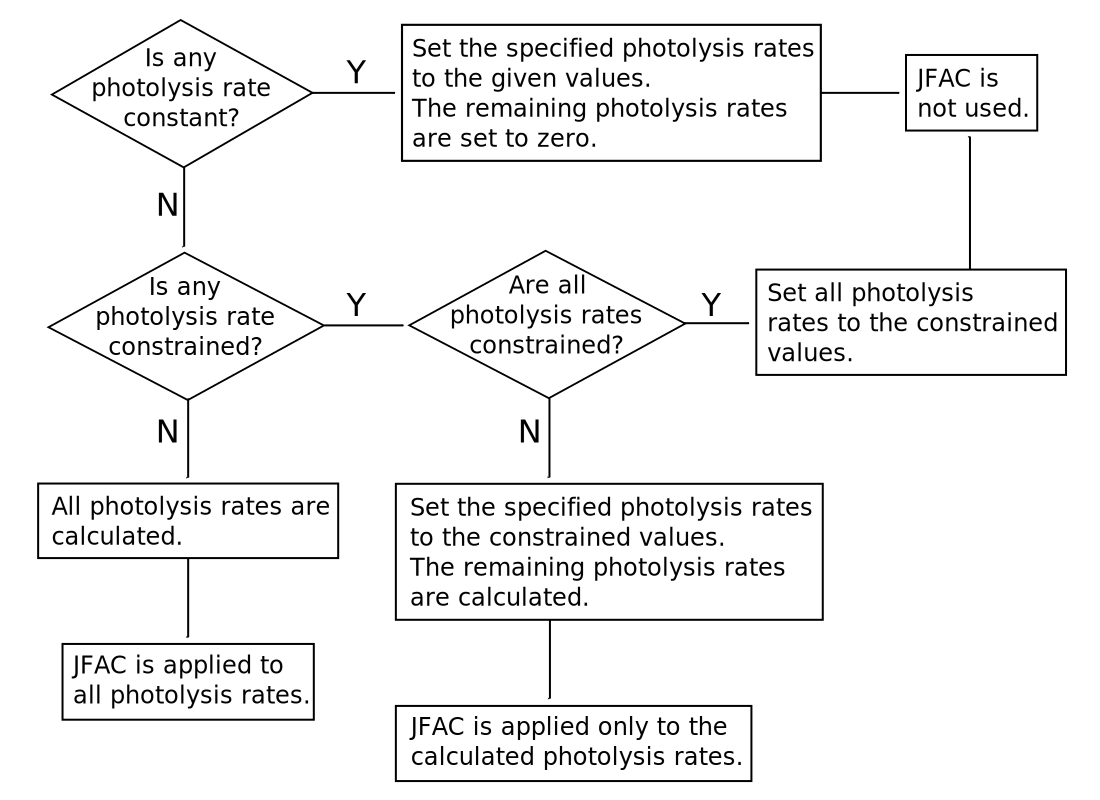
\includegraphics[width=0.85\textwidth]{photolysis-rates.png}
  \caption{Treatment of photolysis rates in AtChem2.}
  \label{fig:photol}
\end{figure}

\subsection{Constant photolysis rates} \label{subsec:constant-photolysis-rates}

The typical scenario for constant photolysis rates is a lamp or solar
simulator in an environmental chamber. All the photolysis rates in the
chemical mechanism must be given a value in the
\texttt{photolysisConstant.config} file, otherwise they are
automatically set to zero (Fig.~\ref{fig:photol}).  This approach
allows the user to model individual photolysis processes and/or to
account for lamps that emit only in certain spectral windows.

The format of \texttt{photolysisConstant.config} is described in
Sect.~\ref{subsec:photolysisconstant}. If the file is empty, the
photolysis rates are calculated or constrained -- see below.

\subsection{Constrained photolysis rates} \label{subsec:constrained-photolysis-rates}

All photolysis rates can be constrained to measured values. In order
to do so, the name of the constrained photolysis rate (e.g.,
\texttt{J2}) must be listed in the
\texttt{photolysisConstrained.config} file
(Sect.~\ref{subsec:photolysisconstrained}); a corresponding file with
the constraint data must be present in the
\texttt{model/constraints/photolysis/} directory
(Sect.~\ref{subsec:constrained-variables}).

It is not always possible to measure -- and therefore to constrain --
all the required photolysis rates. The photolysis rates that are not
constrained (i.e. that are not listed in
\texttt{photolysisConstrained.config}) are calculated using the MCM
parametrization, described in the next section.

\subsection{Calculated photolysis rates} \label{subsec:calculated-photolysis-rates}

AtChem2 implements the parametrization of photolysis rates used by the
Master Chemical Mechanism, which is described in detail in the MCM
protocol papers \citep{jenkin_1997, saunders_2003}. Briefly, the
photolysis rate (\texttt{J}) of a reaction is calculated as a function
of the solar zenith angle with the equation:

\begin{equation}
  J = l \times (cosX)^m \times e^{(-n \times secX)} \times \tau
\end{equation}

where $l$, $m$, $n$ are empirical parameters, $cosX$ is the cosine of
the solar zenith angle, $secX$ is the inverse of $cosX$ (i.e.
$secX\ =\ 1/cosX$) and $\tau$ is the transmission factor. The
transmission factor accounts for the loss of natural or artificial
light in some environmental chambers: the default value of $\tau$ is 1
(i.e. perfect trasmittance of the chamber walls).

The empirical parameters are different for each version of the MCM: by
default, AtChem2 uses the empirical parameters of the MCM v3.3.1
(\texttt{mcm/photolysis-rates\_v3.3.1}), but it is possible to use the
empirical parameters of other versions of the MCM and to change the
value of $\tau$: see the file \texttt{mcm/INFO.md} for instructions.

The solar zenith angle (SZA) is the angle between the local vertical
(zenith) and the center of the sun. The SZA is measured in radians and
is calculated by the model from latitude, longitude, sun declination
(\hyperref[subsec:dec]{\texttt{DEC}}) and time of the day. The
calculations of the sun declination -- if not constrained or set to a
constant values -- and of the solar zenith angle are described in
\citet{madronich_1993}.

\subsection{JFAC calculation} \label{subsec:jfac-calculation}

Measurements of ambient photolysis rates typically show short-term
variability due to changing meteorological conditions, such as clouds,
rain, aerosol, etc\ldots \citep{sommariva_2020}. This information is
retained in the constrained photolysis rates, but it is lost in the
calculated ones. To account for ambient variability the calculated
photolysis rates can be scaled by a constant or time-dependent
correction factor, the environment variable \texttt{JFAC}
(Sect.~\ref{subsec:jfac}), defined as:

\begin{equation}
  \mathrm{JFAC} = \frac{j_{meas}}{j_{calc}}
\end{equation}

where $j_{meas}$ and $j_{calc}$ are the measured and calculated (with
the MCM parametrization, Sect.~\ref{subsec:calculated-photolysis-rates})
photolysis rates of a reference species. \cf{NO2} is often used as a
reference because $j$(\cf{NO2}) is one of the most frequently measured
photolysis rates, in which case: \verb|JFAC = j(NO2)/J4|.

\texttt{JFAC} is by default set to 1, which means that the calculated
photolysis rates are not scaled; \texttt{JFAC} can be set to any value
between 0 and 1 (Sect.~\ref{subsec:jfac}) or it can be constrained
(Sect.~\ref{subsec:constrained-variables}). Note that only the
photolysis rates calculated with the MCM parametrization are scaled by
\texttt{JFAC}: the constrained and the constant photolysis rates are
never scaled (Fig.~\ref{fig:photol}).

\texttt{JFAC} can be calculated by AtChem2 at runtime. To use this
option, edit the \texttt{environmentVariables.config} file
(Sect.~\ref{subsec:environmentvariables}) and set \texttt{JFAC} to the
name of the photolysis rate used as reference (e.g., \texttt{J4}). In
addition, the reference photolysis rate must be constrained -- i.e.
it must be listed in \texttt{photolysisConstrained.config}
(Sect.~\ref{subsec:photolysisconstrained}) and the corresponding
constraint file must be present in the
\texttt{model/constraints/photolysis/} directory~\footnote{The
  calculation of \texttt{JFAC} at runtime does not work well in the
  current version of AtChem2, especially in situations when the
  reference photolysis rate is very variable. Therefore, it is
  recommended to calculate \texttt{JFAC} offline and then to constrain it
  (see issue \href{https://github.com/AtChem/AtChem2/issues/16}{\#16}).}.

% -------------------------------------------------------------------- %
\section{Config Files} \label{sec:config-files}

The configuration files contain the settings of the environment
variables, the chemical species, the photolysis rates, as well as the
model constraints and the model output. All the configuration files
have the extension \texttt{.config} and, by default, are located in
the \texttt{model/configuration/} directory. This directory also
contains the files with the settings of the model
(\texttt{model.parameters}) and of the solver
(\texttt{solver.parameters}), which are described in
Sect.~\ref{sec:model-parameters} and Sect.~\ref{sec:solver-parameters}.

Usually, the \texttt{model/configuration/} directory is also the
\sharedir, which contains the chemical mechanism files generated
during the \hyperref[subsec:build-process]{build process}. The names
and locations of these directories can be modified by the user, as
explained in Sect.~\ref{subsec:model-directory}. The content and the
format of each \texttt{.config} file are described below. Note that
the names of some files have changed with the release of AtChem2
version 1.1 (November 2018).

\subsection{environmentVariables.config} \label{subsec:environmentvariables}

This file contains the settings of the environment variables
(Sect.~\ref{sec:environment-variables}). The file has three columns:
the first two are the ID number and the name of each
environment variable. The third column, which is the only one that
should be modified by the user, contains the settings of the
environment variables. For example:

\begin{verbatim}
1   TEMP         293
2   PRESS        1013
3   RH           CONSTRAINED
4   H2O          CALC
5   DEC          CALC
6   BLHEIGHT     8e+4
7   DILUTE       NOTUSED
8   JFAC         CONSTRAINED
9   ROOF         OPEN
10  ASA          2e-5
\end{verbatim}

If an environment variable is constrained, there must be a
corresponding data file in the \texttt{model/constraints/environment/}
directory (Sect.~\ref{subsec:constrained-variables}).

\subsection{initialConcentrations.config} \label{subsec:initialconcentrations}

This file contains the initial concentrations of the chemical species
-- in molecule cm$^{-3}$. The file has two columns: the first column
is the list of initialized species, the second column is the
corresponding concentration at \texttt{t\ =\ 0}. For example:

\begin{verbatim}
O3      1.213e+12
NO      378473308.14
NO2     86893908168.9
CH4     4.938e+13
\end{verbatim}

Not all chemical species need to be initialized: those that are not
listed in \texttt{initialConcentrations.config} are automatically set
to an initial concentration of 0.0E+00 molecule cm$^{-3}$. It is
\emph{not necessary} to initialize the chemical species that are set
to constant or constrained (i.e. those listed in
\texttt{speciesConstant.config} or in \texttt{speciesConstrained.config}
-- see below).

\subsection{outputRates.config} \label{subsec:outputrates}

This file lists the chemical species for which detailed production and
loss rates are required. In version 1.0 and earlier, these species
were listed in two files called \texttt{productionRatesOutput.config}
and \texttt{lossRatesOutput.config}. The file has one column, with one
species per line. For example:

\begin{verbatim}
OH
HO2
CH3O2
\end{verbatim}

The frequency of this output is controlled by the \textbf{rates output
  step size} parameter in \texttt{model.parameters}
(Sect.~\ref{sec:model-parameters}). The corresponding output files --
called \texttt{productionRates.output} and \texttt{lossRates.output}
-- are designed to facilitate the rate of production and destruction
analysis (ROPA/RODA) of selected species of interests, rather than
processing all the files saved in the \texttt{model/output/reactionRates/}
directory. For more information, go to Sect.~\ref{sec:output}.

\subsection{outputSpecies.config} \label{subsec:outputspecies}

This file (called \texttt{concentrationOutput.config} in version 1.0
and earlier) lists the chemical species for which the calculated
concentration -- in molecule cm$^{-3}$ -- is required. The file has
one column, with one species per line. For example:

\begin{verbatim}
O3
NO
NO2
CH4
OH
HO2
CH3O2
\end{verbatim}

The frequency of this output is controlled by the \textbf{step size}
parameter in \texttt{model.parameters} (Sect.~\ref{sec:model-parameters}).
The constrained chemical species can be listed in
\texttt{outputSpecies.config}, which can be useful for diagnostic and
debugging purposes. Note that the photolysis rates, the environment
variables and the \cf{RO2} sum are always output by the model
(Sect.~\ref{sec:output}) and therefore there is not an equivalent
\texttt{.config} file for the output of these variables.

\subsection{photolysisConstant.config} \label{subsec:photolysisconstant}

This file lists the photolysis rates that are set to constant
(Sect.~\ref{subsec:constant-photolysis-rates}). The file has three
columns: the first column is the ID number of the photolysis rate, the
second column is the value of the photolysis rate (in s$^{-1}$), the
third column is the name of the photolysis rate. The ID numbers and
the names of the photolysis rates follow the
\href{http://mcm.york.ac.uk/parameters/photolysis.htt}{MCM designation}.
For example:

\begin{verbatim}
1     2.5e-5     J1
4     8.7e-3     J4
7     1.8e-3     J7
\end{verbatim}

The photolysis rates that are not listed in
\texttt{photolysisConstants.config} are automatically set to zero
(Fig.~\ref{fig:photol}). If no photolysis rate is set to constant, the
file should be empty.

\subsection{photolysisConstrained.config} \label{subsec:photolysisconstrained}

This file (called \texttt{constrainedPhotoRates.config} in version 1.0
and earlier) lists the photolysis rates that are constrained
(Sect.~\ref{subsec:constrained-photolysis-rates}). The file has one column, with
one photolysis rate per line. The names of the photolysis rates follow the
\href{http://mcm.york.ac.uk/parameters/photolysis.htt}{MCM designation}.
For example:

\begin{verbatim}
J1
J4
J7
\end{verbatim}

If a photolysis rate is constrained, there must be a corresponding
constraint file in the \texttt{model/constraints/photolysis/}
directory (Sect.~\ref{subsec:constrained-variables}). The photolysis
rates that are not listed in \texttt{photolysisConstrained.config} are
calculated using the MCM parametrization (Fig.~\ref{fig:photol}). If
no photolysis rate is constrained, the file should be empty.

\subsection{speciesConstant.config} \label{subsec:speciesconstant}

This file (called \texttt{constrainedFixedSpecies.config} in version
1.0 and earlier) lists the chemical species that are set to
constant. The file has two columns: the first column is the list of
constant species, the second column is the corresponding concentration
-- in molecule cm$^{-3}$. For example:

\begin{verbatim}
CH4     4.4e+13
CO      2.5e+12
H2      1.2e+13
\end{verbatim}

The chemical species that are set to a constant value do not need to
be initialized: the values set in \texttt{speciesConstant.config}
override those set in \texttt{initialConcentrations.config}. If no
chemical species is set to constant, the file should be empty.

\subsection{speciesConstrained.config} \label{subsec:speciesconstrained}

This file (called \texttt{constrainedSpecies.config} in version 1.0
and earlier) lists the chemical species that are constrained. The file
has one column, with one species per line. If a chemical species is
constrained, there must be a corresponding constraint file in the
\texttt{model/constraints/species/} directory
(Sect.~\ref{subsec:constrained-variables}). For example:

\begin{verbatim}
CH4
CO
H2
\end{verbatim}

The chemical species that are constrained do not need to be
initialized: the values set in \texttt{speciesConstrained.config}
override those set in \texttt{initialConcentrations.config}. If no
chemical species is constrained, the file should be empty.
